%%%%%%%%%%%%%%%%%%%%%%%%%%%%%%%%%%%%%%%%%%%%%%%%%%%%%%%%%%%%%%%%%%%%%%%%%%%%%%%%
\chapter{Dynamic Modelling}
%%%%%%%%%%%%%%%%%%%%%%%%%%%%%%%%%%%%%%%%%%%%%%%%%%%%%%%%%%%%%%%%%%%%%%%%%%%%%%%%

This section covers the kinetic modelling of a spacecraft in the vicinity of an
asteroid. Throughout the mathematical description of the considered dynamics,
design choices are motivated with regards their respective effects on simulation
fidelity and computational complexity. The spacecraft's \textbf{rotational
kinetics} can be modelled through the use of Newton's second law applied in the
inertial frame (superscripted as "I") as
$\frac{d}{dt}(\mathbf{I}^I\mathbf{\omega})=\mathbf{M}^I$. This is however not
helpful as $\mathbf{\omega}$ and $I^I$ can change during the motion. Instead it
is preferred to use Euler's equations describing the rotation of a rigid body,
using a rotating reference frame attached to its principal axes of inertia:

\begin{equation}
{\displaystyle \mathbf {I} {\dot {\boldsymbol {\omega }}}+{\boldsymbol {\omega }}\times \left(\mathbf {I} {\boldsymbol {\omega }}\right)=\mathbf {M},}
    \label{eq:euler_rotation}
\end{equation}
\begin{equation*}
    \begin{aligned}
        \textrm{where, }
        \mathbf{I} &= \textrm{the inertia tensor,}\\
        \dot{\mathbf{\omega}} &= \textrm{the angular acceleration vector,}\\
        \mathbf{\omega} &= \textrm{the angular velocity vector,}\\
        \mathbf{M} &= \textrm{the torque vector,}\\
    \end{aligned}
\end{equation*}

Expansion of \autoref{eq:euler_rotation} in three-dimensional principle orthogonal coordinates gives

\begin{equation}
{\begin{aligned}
     I_{1}{\dot  {\omega }}_{{1}}+(I_{3}-I_{2})\omega _{2}\omega _{3}&=M_{{1}},\\I_{2}{\dot  {\omega }}_{{2}}+(I_{1}-I_{3})\omega _{3}\omega _{1}&=M_{{2}},\\I_{3}{\dot  {\omega }}_{{3}}+(I_{2}-I_{1})\omega _{1}\omega _{2}&=M_{{3}}.
\end{aligned}}
\end{equation}

In physical reality, the instantaneous thrust control capabilities of a
spacecraft are heavily dependent upon the current attitude of the spacecraft.
This coupling is key in guidance strategies that ensure mission success in the
short-term, such as docking in spacecraft rendezvous \cite{Hovell2021}. High
model fidelity is always desirable, however the cost of modelling the rotational
kinematics of a spacecraft is an approximate twofold expense in computational
complexity. It is therefore common for the rotational kinematic modelling of a
spacecraft to be assumed as decoupled from the translational kinematics for
long-term horizon guidance and control strategies. Further motivation for the
omission of the rotational kinematics is the \textit{curse of dimensionality}, a
term coined by Richard E. Bellman \cite{bellman1957dynamic}
\cite{bellman1961adaptive}. This phenomena occurs in many domains and can be
described as the effect of increased sparsity when increasing the dimensions of
data, as less volume is filled by the data in the volume spanned by the
increased dimensions. The spacecraft's \textbf{translational kinetics} can be
effectively modelled using Newton's second law in the inertial frame as
$\frac{d}{dt}(m\textbf{v}^I)=\textbf{F}^I$. There are a plethora of forces
incident upon a spacecraft in interplanetary space, however a majority of their
magnitudes are of such a low order that their effects can be considered
negligible in most cases. This coupled with the fact that it is superfluous to
model effects on the spacecraft's kinetics that are of magnitudes lower than
than what is discernible with the navigation sensors. This extends to parameter
estimation in that the magnitude of these effects would be negligible compared
to measurement noise. \autoref{tab:acc_effects} shows the effect of omitting
specific acceleration models on the final state of an asteroid mission with the
approximate parameters taken from the NEAR Shoemaker mission.

\begin{table}
    \caption{
        The effects of different accelerations on the final kinematic state of
        the NEAR Shoemaker spacecraft \textmd{after being integrated with a
        fixed time-step ($dt$) of 100 s, of an interval of one orbital period
        with the initial Keplerian elements ($a=370\textrm{ km}$) at an initial
        epoch at April 30, 2000 UTC (See \autoref{appendix:c}).}
    }
    \centering
    \label{tab:acc_effects}
    \begin{tabular}{lrr}

        Case                     & $|\mathbf{r}_{e}|$ [m] & $|\mathbf{v}_{e}|$ [m/s] \\
        \hline\hline
        Solar radiation pressure & 1.512680e+04           & 4.319262e-02             \\
        Earth point mass         & 1.925349e-02           & 6.218576e-08             \\
        Moon point mass          & 2.371106e-04           & 7.674187e-10             \\
        Jupiter point mass       & 4.783348e-02           & 1.290854e-07             \\
        Mars point mass          & 2.175087e-04           & 6.178106e-10             \\
        Eros point mass          & 2.318650e+06           & 4.782929e-02             \\

    \end{tabular}
\end{table}

It is evident from \autoref{tab:acc_effects} that the most influential effect on
the kinetics of the spacecraft other than the trivial inclusion of the
point-mass acceleration due to Eros within these mission parameters is the solar
radiation pressure (SRP). It is therefore computationally beneficial, with
minimal impact on the holistic result of the control and guidance, to exclude
all sources of acceleration other than thrust, solar radiation pressure and the
gravitational potential of the target asteroid.

As mentioned in \autoref{ssec:frame_rtn}, the use of the RSW frame for thrust
control provides significant insight into the effects incurred on the Keplerian
elements of an orbit. In the same way that the effects of thrust in this frame
provides meaningful insight to an astrodynamicist, it can be postulated that the
learnability may be improved for an arbitrary machine learning algorithm.

% \begin{equation}
%     \ddot{\mathbf{r}}=-2\bm{\omega}\times\dot{\mathbf{r}}-\dot{\bm{\omega}}\times\mathbf{r}-\bm{\omega}\times(\bm{\omega}\times\mathbf{r})+\sum{\mathbf{a}}
% \end{equation}
% \begin{equation*}
%     \begin{aligned}\textrm{where, }
%     \ddot{\mathbf{r}} &= \textrm{the acceleration of the spacecraft,}\\
%     \bm{\omega}       &= \textrm{the angular velocity of the spacecraft,}\\
%     \dot{\bm{\omega}} &= \textrm{the angular acceleration of the spacecraft,}\\
%     \mathbf{a}        &= \textrm{accelerations acting on the spacecraft,}\\
%     2\bm{\omega}\times{\dot{\mathbf{r}}} &= \textrm{Coriolis acceleration,}\\
%     \dot{\bm{\omega}}\times{\mathbf{r}} &= \textrm{Euler acceleration,}\\
%     \bm{\omega}\times(\bm{\omega}\times\mathbf{r}) &= \textrm{centrifugal acceleration,}\\
%     \sum{\mathbf{a}} &= \textrm{sum of accelerations action on the spacecraft.}
%     \end{aligned}
% \end{equation*}


% \begin{equation}
%     \mathbf{v}_B = \mathbf{v}_A + \Omega \cross \mathbf{r}_{B/A} + \mathbf{v}_{B/A} 
%     \label{rel_gen_plane_motion_vel}
% \end{equation}

% \begin{equation}
%     \mathbf{a}_{B} = \mathbf{a}_A + \dot{\mathbf{\Omega}} \cross \mathbf{r}_{B/A} + \mathbf{\Omega} \cross (\mathbf{\Omega}\cross{\mathbf{r}_{B/A}}) + 2\mathbf{\Omega} \cross {\mathbf{v}_{B/A}} + \mathbf{a}_{B/A}
%     \label{rel_gen_plane_motion_acc}
% \end{equation}

\begin{equation}
    \begin{aligned}
        % \frac{d}{dt}(m\textbf{v}^I) & =\textbf{F}^I\\
        \ddot{\mathbf{r}} = \sum{\mathbf{a}}^I &=\mathbf{a}_g^I + \mathbf{a}_{SRP}^I + \mathbf{a}_T^I\\
        &= \mathbf{R}^{I/B}\mathbf{a}_g^{B} + \mathbf{a}_{SRP}^I + \mathbf{R}^{I/RSW}\mathbf{a}_T^{RSW}
    \end{aligned}
\end{equation}

\begin{equation*}
    \begin{aligned}
        \textrm{where, }
        \mathbf{a}^I &= \textrm{an acceleration in the inertial frame (\autoref{ssec:frame_intertial}),}\\
        \mathbf{a}^B &= \textrm{an acceleration in the BCBF frame (\autoref{ssec:frame_bcbf}),}\\
        \mathbf{a}^{RSW} &= \textrm{an acceleration in the RSW frame (\autoref{ssec:frame_rsw}),}\\
        \mathbf{R}^{Q/P} &= \textrm{rotation transformation from a frame P to Q,}\\
        \mathbf{a}_g &= \textrm{the acceleration due to gravity of the asteroid,}\\
        \mathbf{a}_{SRP} &= \textrm{the acceleration due to solar radiation pressure,}\\
        \mathbf{a}_T &= \textrm{the acceleration due to thrust.}\\
    \end{aligned}
\end{equation*}


% 
% \section{Rotation Model}


% The diagonal components
% $I_x \leq I_y \leq I_z$ are then the principal moments of inertia; the
% axes are called the principal inertia axes.

% \textcolor{red}{Design choice:Low order Librations could be considered for binary asteroids.}

% \begin{equation}
%     R^{P/I}=R_z(W)R_x(\pi/2-\delta)R_z(\pi/2+\alpha)
% \end{equation}

%%%%%%%%%%%%%%%%%%%%%%%%%%%%%%%%%%%%%%%%%%%%%%%%%%%%%%%%%%%%%%%%%%%%%%%%%%%%%%%%
\section{Solar Radiation Pressure}
%%%%%%%%%%%%%%%%%%%%%%%%%%%%%%%%%%%%%%%%%%%%%%%%%%%%%%%%%%%%%%%%%%%%%%%%%%%%%%%%

The simplest method of modelling the effect of solar radiation pressure without
consideration for rotational kinetics can be done using a cannonball radiation
model. This model assumes a constant radiation coefficient regardless of the
orientation of the spacecraft with no torque effects. This behaviour is
identical to that of an object that has spherically symmetric mass distribution,
hence the term "cannonball". In inertial space $\{X_I\}$, this model is
expressed as

\begin{equation}
    \mathbf{a}_{SRP}=-\Xi{}P_\Sun{C}_R\frac{A}{m}\frac{\mathbf{r}_{\Sun}}{|\mathbf{r}_\Sun|^3}AU^2
\end{equation}
\begin{equation*}
    \begin{aligned}
        \textrm{where, }
        \Xi &= \textrm{a 0 or 1 value, respectively the state of solar eclipse and incidence,}\\
        C_R &= \textrm{the coefficient of radiation pressure,} \\
        A  &= \textrm{the reference area of solar incidence,} \\
        m & = \textrm{the instantaneous mass of the spacecraft,} \\
        \mathbf{r}_\Sun &= \textrm{the position vector of the Sun relative to the spacecraft,} \\
        AU &= \textrm{an astronomical unit (1.495978707×${10^{11}}$ m).} \\
        P_\Sun &=  \textrm{the solar radiation pressure incident at 1 AU.}
    \end{aligned}
\end{equation*}

The state of whether to spacecraft is in solar eclipse or incidence can be
determined through the combination of two conditions. An additional auxiliary
vector is considered, the position of the Sun with respect to the central body
($\mathbf{R}_\Sun$). The first condition for eclipse is that the spacecraft
orbital position around the central body ($\mathbf{r}_s$) has a component
perpendicular to $\mathbf{R}_\Sun$ ($a$) which exceeds the radius of the central
body ($R_e$). This condition occurs when either the central body or spacecraft
occults the other. A final check for which of these cases occurs is done by
checking with the angle between $\mathbf{R}_\Sun$ and $\mathbf{r}_s$ ($\Psi$) is
acute or obtuse, that latter indicating that solar occultation is occuring for
the spacecraft.

\begin{figure}[h]
    \centering
    \def\svgwidth{0.8\linewidth}
    % \input{graphics/drawing2.pdf_tex}
    \import{graphics/}{drawing2.pdf_tex}
    \caption{
        Illustration showing the geometry of a solar eclipse with respect to an
        orbiting spacecraft. \textmd{The diagram is represented as a 2D
        cross-section parallel to the orbital plane.}
    }
    \label{fig:my_label}
\end{figure}

The cosine of $\Psi$ is determined and the sine of $\Psi$ follows directly
through trigonometric identities:

\vspace{3mm}
\begin{minipage}{.5\linewidth}
    \begin{equation}
        \cos{\Psi} = \frac{\mathbf{R}_\Sun \cdot \mathbf{r}_s }{|\mathbf{R}_\Sun|| \mathbf{r}_s|},
    \end{equation}
\end{minipage}%
\begin{minipage}{.5\linewidth}
    \begin{equation}
        \sin{\Psi} = \sqrt{1-\cos^2{\Psi}}.
    \end{equation}
\end{minipage}
\vspace{1mm}

The combination of both conditions such that $\Xi$ indicates the incidence of
solar pressure on the spacecraft in logical operator notation is,

\begin{equation}
    \Xi=\lnot((\cos{\Psi}<0)\land(r_s\sin{\Psi}<R_e)).
\end{equation}

It should be noted that that is a simplification of reality, where in fact
there are the regions of the umbra, penumbra and antumbra during eclipse, in
decreasing order of solar incidence.

%%%%%%%%%%%%%%%%%%%%%%%%%%%%%%%%%%%%%%%%%%%%%%%%%%%%%%%%%%%%%%%%%%%%%%%%%%%%%%%%
\section{Thrust}
%%%%%%%%%%%%%%%%%%%%%%%%%%%%%%%%%%%%%%%%%%%%%%%%%%%%%%%%%%%%%%%%%%%%%%%%%%%%%%%%

The kinetics of the spacecraft are dependent on its instantaneous mass, seen in
Newton's second law. The rate of change of mass of the spacecraft is given by
the classical rocket equation

\begin{equation}
    \dot{m}=-\frac{T}{I_{sp}\cdot{g_0}}
\end{equation}
\begin{equation*}
    \begin{aligned}
        \textrm{where, }
        I_{sp} &= \textrm{the specific impulse of the propulsion system,}\\
        T &= \textrm{the net thrust supplied by the propulsion system,}\\
        g_0 &= \textrm{the standard gravity, which is nominally the gravity at Earth's surface.}
    \end{aligned}
\end{equation*}

The acceleration contribution due to thrust is then

\begin{equation}
    \mathbf{a}_T = \frac{\mathbf{T}}{m}.
\end{equation}


%%%%%%%%%%%%%%%%%%%%%%%%%%%%%%%%%%%%%%%%%%%%%%%%%%%%%%%%%%%%%%%%%%%%%%%%%%%%%%%%
\section{Gravitational Potential}
%%%%%%%%%%%%%%%%%%%%%%%%%%%%%%%%%%%%%%%%%%%%%%%%%%%%%%%%%%%%%%%%%%%%%%%%%%%%%%%%

The acceleration due the gravitational potential of a body in inertial space $\{X^I\}$ is expressed as,


\begin{equation}
    \begin{aligned}
        \mathbf{a}_g^I &= \mathbf{R}^{I/B}\nabla_{\mathbf{r}}U(\mathbf{r}^B)\\
        \textrm{replacing \autoref{eq:bci_transformation}:}\;\;\mathbf{a}_g^I &=  \mathbf{R}_z(W)\mathbf{R}_x(\pi/2-\delta_0)\mathbf{R}_z(\pi/2-\alpha_0)\nabla_{\mathbf{r}}U(\mathbf{r}^B)
        \label{eq:accel_grav_pot}
    \end{aligned}
\end{equation}
\begin{equation*}
    \begin{aligned}
        \textrm{where, }
        \nabla_{\mathbf{r}}U(\mathbf{r}) &= \textrm{the vector differential of the gravitational potential field,} \\
        W &= \textrm{the ephemeris position of the prime meridian (\autoref{eq:ephem_prime_meridian}),}\\
        \alpha_0, \delta_0 &= \textrm{ICRF equatorial coordinates (right ascension \& declination) at epoch J2000.0.} \\
    \end{aligned}
\end{equation*}

The transformation from body-fixed coordinates into the inertial frame is
emphasised in \autoref{eq:accel_grav_pot} to make clear the temporal coupling of
a potential field in inertial space. For a spherically symmetric potential, such
as the point mass approximation, only the relative position to the body in
inertial space is needed. This coupling plays a part in defining the equator of
date and the ephemeris position of the prime meridian, which together define the
body-fixed coordinate system of the considered body. When the evolution of the
rotation axis is ignored, this coupling results in five base characteristic
parameters of the gravitational potential field in inertial space when
processing Earth-based observations: $W_0$, $\dot{W}$, $\alpha_0$, $\delta_0$
and $\mathbf{r}^{I/B}$. For the remainder of this section on gravitational
potential, the body-fixed coordinate $\mathbf{r}^B$ will be referred to as
$\mathbf{r}$ for simplicity. As noted by by Montenbruck & Gill
\cite{Montenbruck2000}, the gravitational potential may be generalised to an
arbitrary mass distribution through the summation of all contributions of
individual mass elements, with $dm=\rho{(\mathbf{r'})}d^3\mathbf{r'}$,

\begin{equation}
    U(\mathbf{r}) = G\int_V\ frac{\rho{(\mathbf{r'})}}{|\mathbf{r}-\mathbf{r'}|}\;d^3\mathbf{r'}
\end{equation}
\begin{equation*}
    \begin{aligned}
        \textrm{where, }
        G &= \textrm{the universal gravitational constant }(6.6695\times{}10^{−11} [\textrm{m}^3\cdot{}\textrm{kg}^{-1}\cdot{}\textrm{s}^{-2}])\\
        \mathbf{r}       &= \textrm{position at which potential is calculated,} \\
        \mathbf{r'}       &= \textrm{position of point inside the body mass,}\\
        \rho(\mathbf{r'}) &= \textrm{density at given point inside the body mass.}
    \end{aligned}
\end{equation*}

The acceleration contribution due to gravity is related to gravitational
potential through $\mathbf{a}_g=\nabla_\mathbf{r}{U}$.

%%%%%%%%%%%%%%%%%%%%%%%%%%%%%%%%%%%%%%%%%%%%%%%%%%%%%%%%%%%%%%%%%%%%%%%%%%%%%%%%
\subsection{Point mass}
%%%%%%%%%%%%%%%%%%%%%%%%%%%%%%%%%%%%%%%%%%%%%%%%%%%%%%%%%%%%%%%%%%%%%%%%%%%%%%%%

The lowest fidelity gravitational potential model that can be used in estimation
is a point-mass approximation to gravitational potential,

\begin{equation}
    U(r)=\frac{GM}{r}
\end{equation}

\begin{equation*}
    \begin{aligned}
        \textrm{where, } M &= \textrm{mass of the primary body generating the potential field.}
    \end{aligned}
\end{equation*}

This model has the main advantage that it is decoupled from the body-fixed
coordinate system, reducing the number of estimated parameters required for a
first order approximation of the mass of a the considered body. The acceleration
contribution due to gravity is then,

\begin{equation}
    \bm{a}_g=
    \begin{bmatrix}
        a_{g_x} \\
        a_{g_y} \\
        a_{g_z}
    \end{bmatrix}
    =
    \nabla_\mathbf{r}{U}
    =
    \begin{bmatrix}
        \frac{\partial{U}}{\partial{x}} \\
        \frac{\partial{U}}{\partial{y}} \\
        \frac{\partial{U}}{\partial{z}}
    \end{bmatrix}
    =
    \begin{bmatrix}
        -\frac{GM}{{r_x}^2} \\
        -\frac{GM}{{r_y}^2} \\
        -\frac{GM}{{r_z}^2}
    \end{bmatrix}
\end{equation}

% \begin{aligned}

%     a_{g_x}=\frac{\partial{U}}{\partial{x}} &= -\frac{GM}{{r_x}^2} \\
%     a_{g_y}=\frac{\partial{U}}{\partial{y}} &= -\frac{GM}{{r_y}^2} \\
%     a_{g_z}=\frac{\partial{U}}{\partial{z}} &= -\frac{GM}{{r_z}^2} \\
% \end{aligned}
% \begin{equation}
%     \mathbf{a}_g(\mathbf{r})=-\frac{GM}{r^3}\mathbf{r}
% \end{equation}

%%%%%%%%%%%%%%%%%%%%%%%%%%%%%%%%%%%%%%%%%%%%%%%%%%%%%%%%%%%%%%%%%%%%%%%%%%%%%%%%
\subsection{Tri-axial ellipsoid: elliptical integrals\label{subsub:tri_axial_ellipsoid}}
%%%%%%%%%%%%%%%%%%%%%%%%%%%%%%%%%%%%%%%%%%%%%%%%%%%%%%%%%%%%%%%%%%%%%%%%%%%%%%%%

An alternative lower fidelity model of a body is the use of a tri-axial
ellipsoid of homogenous mass distribution. This approach assumes the small
body's density ($\rho$) as uniform, which allows the gravitational parameter
($\mu$) of the body to be expressed as,

\begin{equation}
    \mu=GM=G\rho\frac{4}{3}\pi{abc}.
\end{equation}

\begin{figure}[h]
    \centering
    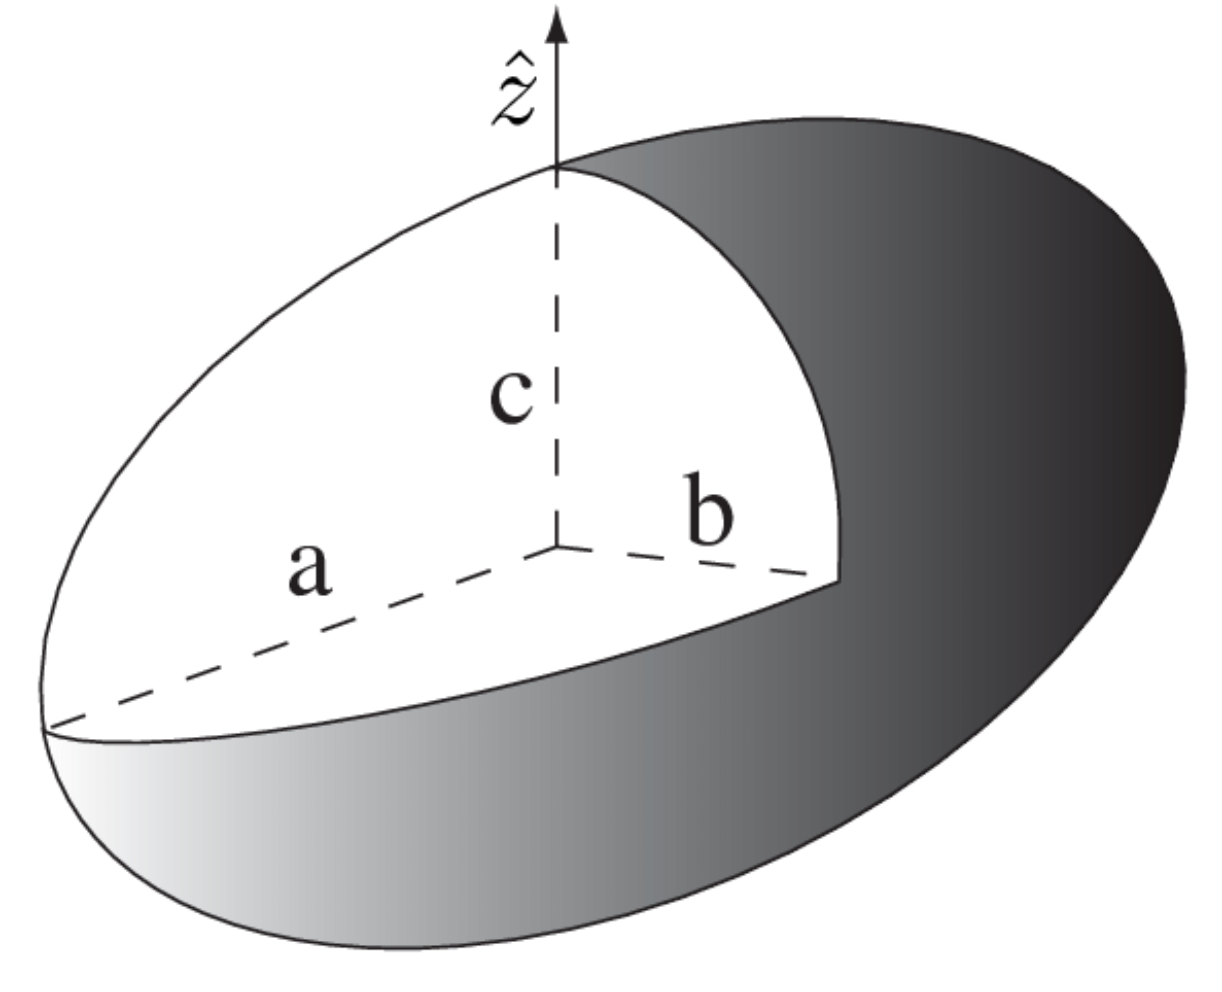
\includegraphics[width=0.35\linewidth]{graphics/tri-axial.png}
    \caption{Tri-axial ellipsoid model \textmd{of homogeneous mass distribution $\rho$, with $I_x<I_y<I_z$, respectively with axes a, b, and c.}}
    \label{fig:tri-axial-model}
\end{figure}

This model is illustrated in \autoref{fig:tri-axial-model} with $I_x<I_y<I_z$.
This model corresponds to the convention of body-fixed frames which have their
$Z$-axis aligned with the rotational axis of the body, however due to precession
and nutation, the true $Z$-axis of date representing the current rotation axis
will differ from the geometrical $\hat{Z}$-axis of the tri-axial ellipsoid. The
period of precession and nutation for short time scales however can be omitted
and for studies which does not involve long term analysis of the subsequent
effects, $Z\approx{\hat{Z}}$. There is a closely related model which is the next
step taken by astrodynamacists after a point mass approximation in missions
design, which is the use of an oblate spheroid. This is often used to account
for the mass concentration at the equator of Earth. This model is obtained from
the homogeneous tri-axial ellipsoid by simply setting $b=a$. The gravitational
potential, $U$, using this model with elliptical integrals, of a body in its
body-fixed reference frame $\{X^B\}$ is

\begin{equation}
    U(\mathbf{r})=\frac{3}{4}\mu \int_{\kappa_0}^{\infty}\bigg(1-\frac{{r_x}^2}{a^2+\kappa} - \frac{{r_y}^2}{b^2+\kappa} - \frac{{r_z}^2}{c^2+\kappa}\bigg)\cdot{}\frac{d\kappa}{\sqrt{((a^2+\kappa)(b^2+\kappa)(c^2+\kappa))}}
    \label{eq:triaxial_ellipsoid_potential_elliptic_integral}
\end{equation}

\begin{equation*}
    \begin{aligned}
        \textrm{where, }
        \kappa &= \textrm{parameter of the pencil for a confocal ellipse}\\
        \kappa_0 &= \textrm{largest root of the confocal ellipsoid}\\
        a, b, c &= \textrm{length of ellipsoid axes, respectively in the x, y and z directions of the body-fixed frame $\{X^B\}$.}
    \end{aligned}
\end{equation*}

\begin{equation}
    C(\kappa) = \frac{{r_x}^2}{a^2+\kappa} + \frac{{r_y}^2}{b^2+\kappa} + \frac{{r_z}^2}{c^2+\kappa} - 1.
\end{equation}

The expressions above are attributed to \cite{Ivory1809}, a detailed derivation
is given by Mac Millan \cite{MacMillan1958}, Danby \cite{Danby1992} and Moulton
\cite{moulton1970introduction}. The integrals seen in
\autoref{eq:triaxial_ellipsoid_potential_elliptic_integral} are elliptic
integrals. By use of Legendre's canonical elliptic integrals of first kind $F$
and second kind $E$, it is possible to find an expression for $U$ and it's
derivatives. Alternatively, as demonstrated by Willis et al. \cite{Willis2016},
a more modern approach using Carlson elliptic integrals. After introducing
$\kappa'=\kappa-\kappa_0$ in
\autoref{eq:triaxial_ellipsoid_potential_elliptic_int}, the gravitational
potential becomes,

\begin{equation}
    \begin{aligned}
        U(\mathbf{r}) &= \frac{3}{2}\mu{R_F}(a^2+\kappa_0, b^2 + \kappa_0, c^2 + \kappa_0)\\
        &- \frac{1}{2}\mu{{r_x}^2}R_D(b^2 + \kappa_0, c^2+\kappa_0, a^2+\kappa_0)\\
        &- \frac{1}{2}\mu{{r_y}^2}R_D(a^2 + \kappa_0, c^2+\kappa_0, b^2 + \kappa_0)\\
        &- \frac{1}{2}\mu{{r_z}^2}R_D(a^2 + \kappa_0, b^2 + \kappa_0, c^2 + \kappa_0),
    \end{aligned}
\end{equation}


where $R_F(x, y, z)$ and $R_{D}(x, y, z)$ are two of the Carlson symmetric forms, and their incomplete elliptic integrals are

\begin{equation}
    R_F(x, y, z) = \frac{1}{2}\int_0^\infty\frac{dt}{\sqrt{(t+x)(t+y)(t+z)}},
    \label{eq:r_f}
\end{equation}
\begin{equation}
    R_D(x, y, z) = \frac{3}{2}\int_0^\infty\frac{dt}{(t+x)\sqrt{(t+x)(t+y)(t+z)}}.
    \label{eq:r_d}
\end{equation}

The numerical evaluation of the above expressions (\autoref{eq:r_f} and
\autoref{eq:r_d}) are detailed by Johansson \cite{Johansson2019}. The
acceleration due to the gravitational potential then becomes:

% \begin{equation}
%     \begin{aligned}
%     a_{g_x} = \frac{\partial{V}}{\partial{x}} = \mu{r_x}{R_D(b^2 + \kappa_0, c^2 + \kappa_0, a^2 + \kappa_0)}\\
%     a_{g_y} = \frac{\partial{V}}{\partial{y}} = \mu{r_y}{R_D(a^2 + \kappa_0, c^2 + \kappa_0, b^2 + \kappa_0)}\\
%     a_{g_z} = \frac{\partial{V}}{\partial{y}} = \mu{r_z}{R_D(a^2 + \kappa_0, b^2 + \kappa_0, c^2 + \kappa_0)}\\
%     \end{aligned}
% \end{equation}
\begin{equation}
    \bm{a}_g
    =
    \begin{bmatrix}
        a_{g_x} \\
        a_{g_y} \\
        a_{g_z}
    \end{bmatrix}
    =
    \nabla_\mathbf{r}{U}
    =
    \begin{bmatrix}
        \frac{\partial{U}}{\partial{x}} \\
        \frac{\partial{U}}{\partial{y}} \\
        \frac{\partial{U}}{\partial{z}}
    \end{bmatrix}
    =
    \begin{bmatrix}
        \mu{r_x}{R_D(b^2 + \kappa_0, c^2 + \kappa_0, a^2 + \kappa_0)} \\
        \mu{r_y}{R_D(a^2 + \kappa_0, c^2 + \kappa_0, b^2 + \kappa_0)} \\
        \mu{r_z}{R_D(a^2 + \kappa_0, b^2 + \kappa_0, c^2 + \kappa_0)} \\
    \end{bmatrix}
\end{equation}


%%%%%%%%%%%%%%%%%%%%%%%%%%%%%%%%%%%%%%%%%%%%%%%%%%%%%%%%%%%%%%%%%%%%%%%%%%%%%%%%
\subsection{Expansion in spherical harmonics}
%%%%%%%%%%%%%%%%%%%%%%%%%%%%%%%%%%%%%%%%%%%%%%%%%%%%%%%%%%%%%%%%%%%%%%%%%%%%%%%%

The general approach for high fidelity gravitational potential modelling is the
use of spherical harmonic expansion. The gravitational potential, $U$, of a
body, in its body-fixed reference frame $\{X^B\}$ is described by the infinite
series

\begin{equation}
    U(r,\phi,\lambda) = \frac{GM}{r}\sum_{n=0}^\infty{}\sum_{m=0}^n{}\bigg[\bigg(\frac{R}{r}\bigg)^l\times{}\overline{P}_{nm}(\sin{\phi})(\overline{C}_{nm}\cos{m\lambda}+\overline{S}_{nm}\sin{m\lambda})\bigg],
    \label{eq:grav_sh}
\end{equation}
\begin{equation*}
    \begin{aligned}
        \textrm{where, }
        r, \phi, \lambda &= \textrm{spherical coordinates in $\{X^B\}$, respectively the radius coordinate, latitude and longitude,} \\
        G &= \textrm{universal gravitational constant,} \\
        M &= \textrm{mass of body,} \\
        n, m &= \textrm{respectively the degree and order of a particular spherical harmonic,} \\
        R &= \textrm{reference radius,} \\
        \overline{P}_{nm} &= \textrm{the normalized associated Legendre polynomials,} \\
        \overline{C}_{nm}, \overline{S}_{nm} &= \textrm{the normalized spherical harmonic coefficients,} \\
    \end{aligned}
\end{equation*}

This expansion is infinite in priciple and may be truncated in practice
depending on the degree of knowledge of the body surface or gravitational
potential field. The degree and order to which the spherical harmonics are
expanded are determined by the quantity and quality of empirical observations.
These observations constrain the the certainty associated to the harmonic
coefficients in the expansion. The general approach is to fit higher fidelity
expansions, until the residual error between observation and model converge
towards a random normal distribution. This convergence suggests that only
stochastic error sources remain, which cannot be modelled deterministically.
These error sources are usually due to the limitation of the hardware employed
in the collection of measurements.

% Recent models for the Earth, Venus and Mars shapes, complete to degree 1080, 720, and 720 respectively, have been recently
% determined (Balmino, 1993); a model of degree 12 exists for the Moon (Bills
% and Ferrari, 1977) and a model of degree 8 has been established for Phobos by
% Duxbury (1991).

%%%%%%%%%%%%%%%%%%%%%%%%%%%%%%%%%%%%%%%%%%%%%%%%%%%%%%%%%%%%%%%%%%%%%%%%%%%%%%%%
\subsection{Tri-axial ellipsoid: expansion in spherical harmonics}
%%%%%%%%%%%%%%%%%%%%%%%%%%%%%%%%%%%%%%%%%%%%%%%%%%%%%%%%%%%%%%%%%%%%%%%%%%%%%%%%

The expansion in spherical harmonics may be easily expanded to represent a
homogeneous distribution of mass as a tri-axial ellipsoid, providing a bridge to
the elliptic integral representation presented previously. This expansion is
demonstrated by Balmino \cite{Geodesy1994}. After introducing the mass
$M=\frac{4}{3}\pi{abc\rho}$, it is demonstrated that,

\begin{equation}
    \begin{aligned}
        C_{2l,2m}&=\frac{3}{R^{2l}}\frac{l!(2m)!}{2^{2l}(2l+3)(2l+1)!}(2-\delta_{0m})\frac{(2l-2m)!}{(2l + 2m)!}\\
        &\times \sum_{k=0}^{l-m}\frac{(-1)^k(4l-2k)!}{(2l-k)!(2l-2m-2k)!}\\
        &\times
        \sum_{s=0}^{m}\frac{(-1)^s}{(2s)!(2m-2s)!}\sum_{p=0}^k\frac{(2l-2m-2p)!}{(l-m-p)!(k-p)!}\\
        &\times
        \sum_{q=0}^{p}\frac{(2s+2p-2q)!(2m-2s+2q)!}{q!(p-1)!(s+p-q)!(m-s+q)!}\\
        &\times a^{2(m-s+q)}b^{2(s+p-q)}c^{2(l-m-p)},
    \end{aligned}
\end{equation}

where, for example, it is found that,
\begin{equation}
    \begin{aligned}
        C_{20}&=\frac{1}{5R^2}\bigg(c^2-\frac{a^2+b^2}{2}\bigg),\\\vspace{3mm}
        C_{22}&=\frac{1}{20R^2}(a^2-b^2),\\\vspace{3mm}
        C_{40}&=\frac{15}{7}(C_{20}^2+2C_{22}^2),\\\vspace{3mm}
        C_{42}&=\frac{5}{7}C_{20}C_{22},\\\vspace{3mm}
        C_{44}&=\frac{5}{28}C_{22}^2.\\\vspace{3mm}
    \end{aligned}
\end{equation}

It is further noted by Balmino \cite{Geodesy1994} that there is a uniform
convergence condition for \autoref{eq:grav_sh} in the case of the homogenous
tri-axial ellipsoid equivalent expansion, which is $a<c\sqrt{2}$.

% \begin{equation}
%     \begin{aligned}
%     \overline{P}_{nm}(u) &= (1-u^2)^{m/2}\frac{d^m}{du^m}P_n(u)\\
%     \overline{C}_{nm} &= \\
%     \overline{S}_{nm} &= \\
%     \overline{P}_n(u) &= \frac{1}{2^{n}n!}\frac{d^n}{du^n}(u^2-1)^n\\
%     \end{aligned}
% \end{equation}

% \subsection{Expansion in spheroidal harmonics}

% \begin{equation}
%     V(r, \theta, \lambda) = 
% \end{equation}


% \section{Measurement Uncertainty}

% \begin{equation}
%     s_i = s_i + s_i · N(0, \sigma_{SN})
% \end{equation}
